\documentclass[a4paper]{apa6}

\usepackage[english]{babel}
\usepackage[utf8x]{inputenc}
\usepackage{amsmath}
\usepackage{amssymb}
\usepackage{graphics}
\usepackage[colorinlistoftodos]{todonotes}

\title{Corn Field Conditions Time Series Predictions}
\shorttitle{Time Series: Corn}
\author{Joseph Brown \& Jon Stewart}
\affiliation{Data Mining Final}

\begin{document}
\maketitle
\section*{Project Goals}
We had two main objectives for this project. We used two data sets: a data set consisting of weekly corn field conditions, and a data set of corn yield for each year. We wanted to know whether, given a history of field conditions, we could predict future field conditions. Second, given a history of those field conditions, could we predict another, related variable such as corn yields? Each of these involved several models. To predict future field conditions, we used neural networks, ARIMA models, and support vector machines. To predict corn yields, we used neural networks and a random forest algorithm.

\section*{The Data}
The data sets that we used were weekly corn field conditions, as reported by farmers, and corn yields. We took this data from the year 2000 to 2015. The data set of corn field conditions contains at least twenty weeks recorded for each year. Each farmer polled has the option of listing their field conditions as excellent, fair, good, poor, and very poor. For each condition, the data value column of the data set contained the percentage of fields in that condition.  These percentages were rounded to the nearest integer.  Although this could suggest the possibility of Markov chain modeling, since predicted values can be described in terms of discrete values, this is not a great approach since the data shows nonlinear trends, and is not stationary. Since this memoryless assumption is not true --- poor conditions for a given field for many consecutive weeks indicates an increased likelihood of poor conditions for that given field in future weeks --- we could not use this model. The data is recorded over time, making it a natural candidate for time series prediction problems.

These time series also have interesting features. They display non-stationary and periodic behavior. For the corn yield data set, each year’s yield is given. As a time series problem, and treating all the categories as predictor variables, we have a multivariate time series.  Treating each category as the single predictor variables and applying each category to an individual model is another way to approach this problem. Where appropriate we tried both or whichever representation was appropriate for a given model.
One of the immediate problems we ran into is that we did not have enough time series to run as samples. As a counter to this, we used a form of bootstrapping called maximum entropy bootstrapping. Regular bootstrapping with replacement can destroy the correlations and time dependent behavior of the data. Maximum entropy bootstrapping does not have this shortfall, and still allows us to create a large set of time series to work with. This has the effect of allowing us to decrease the variance in our predictions. In a general sense, this is a form of bagging. Altogether, including both the bootstrapped and original time series, we had 1515 time series. Before applying the data to the neural network or random forest algorithms, all of the predictor variables were normalized. Additionally, on the neural networks, a version of the data where a discrete Haar wavelet transform was applied to the model. 

\section*{Performance Metrics}
We used several statistics to track performance. For corn yield prediction, we used the mean squared error of the residuals between the predicted and actual corn yield. We also kept track of the highest and lowest residual. For forecasts of weekly field conditions, we used the same metrics, applied to the residuals by week on the predicted and actual week field conditions, given the previous data. 

\section*{ARIMA Model}
Another model we used specifically for predicting future corn field conditions is an ARIMA model. Since ARIMA is a univariate model for time series, we fit a model for each field condition.	 For ARIMA, determining which lags are significant is important before actually being able to predict future time series. For all of these, we found that lags 1 and 2 with respect to the history of the field condition values were important, while the residuals of the first lag was important for the models Good and fair. Interestingly, lag 11 was also found to be significant. One difficulty we ran into was finding transformations that were able to remove any patterns in the data. This is an important step, otherwise predictions are likely to be disproportionately influenced by large structures.  Further features of the data set which have a negative impact on ARIMA models are:
\begin{itemize}
\item Discontinuities between the first week of each year and the last week of the year prior.
\item Categories of field conditions.
\item Seasonality
\end{itemize}

For each category, we had the following results:
\begin{center}
\begin{tabular}{|r|l|}
  \hline
Excellent & 0.513 \\
Good & 0.745\\
Fair & 0.775\\
Poor & 0.892\\
  \hline
\end{tabular}
\end{center}

For these models, Excellent and Poor were the best predictors of future Excellent and Poor field conditions. (Figures 1 and 2)
\begin{figure}
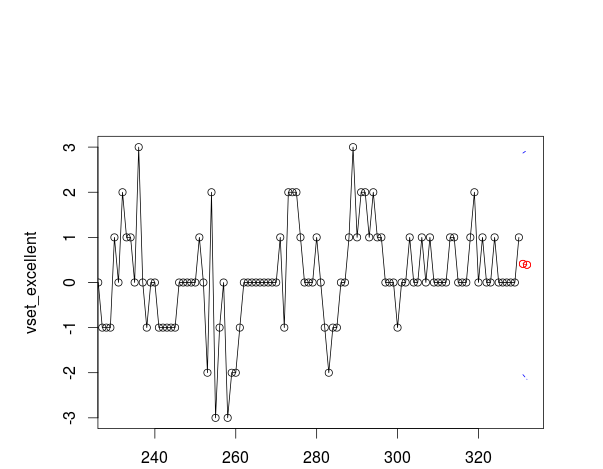
\includegraphics[width=0.8\linewidth]{excellent.png}
\caption{}
\end{figure}
\begin{figure}
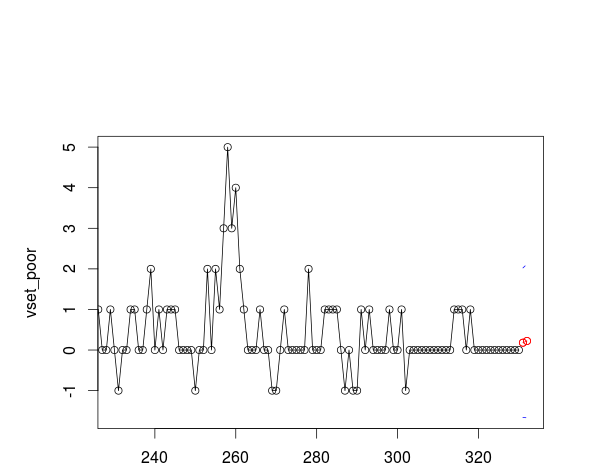
\includegraphics[width=0.8\linewidth]{poor.png}
\caption{}
\end{figure}

It is interesting that ARIMA was better able to predict the more extreme field conditions. Perhaps this was due to more difficulties removing non stationary features from the data. Though the particulars are uncertain, investigating the exact causes are beyond the scope of this project.  Here, the ARIMA models serve only as a benchmark for other models.

\section*{Support Vector Machines}
Support vector machines were vastly superior to the Arima models.  The ability to take into account other field condition categories for the purposes of making predictions was a significant advantage.  To set up the SVM models, lag-matrices were created.  These served as design matrices with past values as additional variables.  Lags of two, and three were both investigated.  The models were tuned individually for optimal gamma and costs.

For each field category, an evaluative plot was created on a model and a set of testing data, constructed with past variables in order to preserve the time-series structure.  The line traces the actual values, and the points are a week-by-week prediction of the next value. (Figures 3-7).  Blue points are within the RMSE of the actual values, while red points are in excess.  These form a very close fit for all field condition categories.

\begin{center}
\begin{tabular}{|r|r|r|r|r|r|}
  \hline
& V.Poor & Poor & Fair & Good & Exct. \\
\hline
RMSE & 1.40 & 1.73 & 1.58 & 3.39 & 1.86 \\
MAE & 0.71 & 0.93 & 0.99 & 1.74 & 1.16 \\
MAX & 6.23 & 7.50 & 3.25 & 4.24 & 6.82 \\
MIN & -2.08 & -2.72 & -5.08 & -15.72 & -3.26\\
  \hline
\end{tabular}
\end{center}

\begin{center}
\begin{figure}
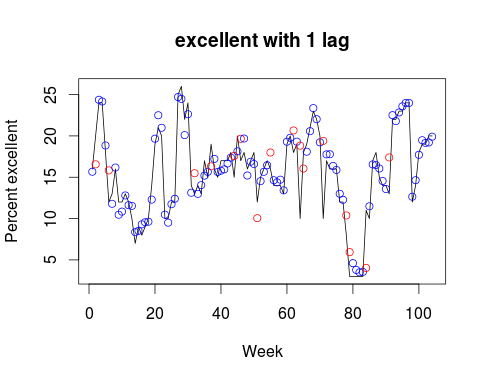
\includegraphics[width=0.8\linewidth]{excellentlag1.png}
\caption{}
\end{figure}
\begin{figure}
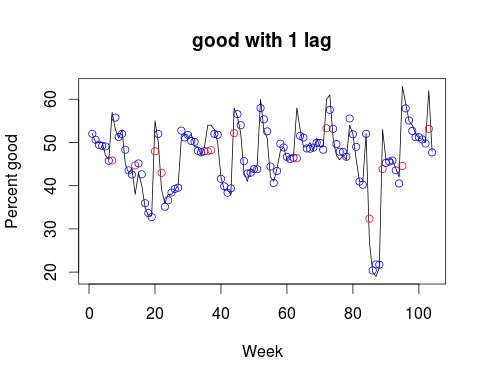
\includegraphics[width=0.8\linewidth]{goodlag1.png}
\caption{}
\end{figure}
\begin{figure}
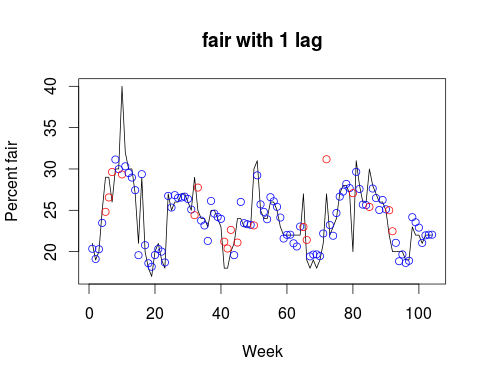
\includegraphics[width=0.8\linewidth]{fairlag1.png}
\caption{}
\end{figure}
\begin{figure}
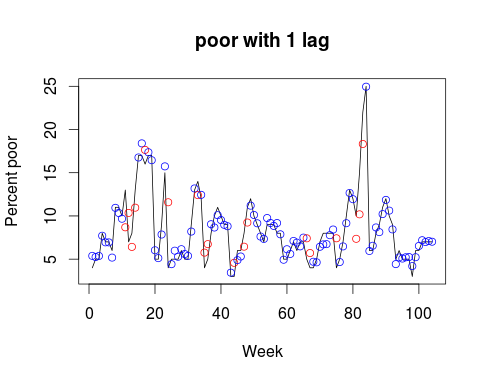
\includegraphics[width=0.8\linewidth]{poorlag1.png}
\caption{}
\end{figure}
\begin{figure}
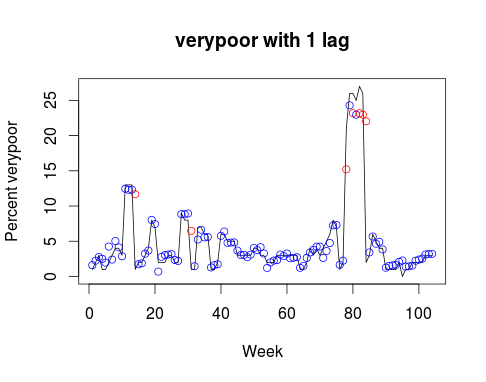
\includegraphics[width=0.8\linewidth]{verypoorlag1.png}
\caption{}
\end{figure}
\end{center}


\section*{Haar Wavelet Transform}
A Haar Wavelet Transformation was applied to remove noise from the data.  A neural network trained on this transformation was then compared to a neural network with normalized data.  

\section*{Random Forest}
An additional model that we used for predicting corn yield was a random forest algorithm. For this, we chose not to use the wavelet transformed data, and only used the normalized data set. This was due to the fact that we were unsure how to directly apply and interpret the wavelet transformed data. A wavelet transformed data set projects a series in time to both a time and frequency space. It was unclear how a decision tree applies this. For the random forest algorithm, we tried several different formats. First, we tried each field condition as a separate predictor of corn yield. For this we got the following MSE values:

\begin{center}
\begin{tabular}{|r|r|r|r|r|}
  \hline
&  Poor & Fair & Good & Exct. \\
\hline
MSE & 51.48 & 0.36 & 1.10 & 0.69 \\
  \hline
\end{tabular}
\end{center}



Here, Fair was clearly the best individual predictor of corn yield. Next, we tried to combine predictions in different ways. Creating an unweighted entry wise average of the predictions, we got a model error of 280.0846. Next, we tried using a model with a weighted average such that each individual predictor was weighted by it’s training mean squared error. It was important to use the training mean squared error rather than the testing mean squared error otherwise we would make inaccurate inferences regarding the model’s ability to predict a new year’s corn yield. 

\section*{Neural Networks}
The first goal was to see how well a neural network with the wavelet transformed data was able to predict corn yields. After fitting the model for the optimal net size, we then tested out the model. We obtained an MSE of 35.28519 and a min and max residual of 0.001400698 and 16.57528 respectively. In comparison, the non-wavelet transformed data had an MSE of 153.4402 and a min and max residual of 0.2827361 and 25.08274 respectively. The wavelet transformed data performed much better in regards to neural network time series prediction. 
Next, we wanted to see how well we could predict future weekly field conditions. For these, we wanted to see how well a category is able to predict that category in future weeks. For neural networks, we were able to run this for one and two weeks ahead. Each individual model was fit so the neural network size was optimal for each model.  For this data, since the discrete wavelet transformed data was clearly superior to the data that was only normalized, we only did the discrete wavelet transforms. For each sample one week ahead, we got the following MSE scores:

\begin{center}
\begin{tabular}{|r|r|r|r|r|}
  \hline
&  Poor & Fair & Good & Exct. \\
\hline
MSE & 51.48 & 0.36 & 1.10 & 0.69 \\
  \hline
\end{tabular}
\end{center}

Excellent    0.868548

Good	      1.407413

Fair 	      0.1672067

Poor	      0.3661849

For two steps ahead, I obtained:

Excellent    1.111419

Good	      1.362944

Fair	      0.1331234

Poor	      0.4052716

From these results, it seems that Fair field conditions are the best predictor of future values of fair field conditions. This is true for both one and two steps ahead. Interestingly, the fair field conditions actually have a slightly better mean square error for predicting two weeks into the future. Excellent and good categories tend to do the worst at predicting future values of good and excellent. 

\section*{Comparison of Models}
	
There are two explicit types of time series prediction performed in our project. First, we tried to predict future field conditions, given a previous history of field conditions. The second type of time series regression we performed was, given a time series of field conditions, could we predict another variable? In this, case, we wanted to predict corn yield. The reasoning for this was two-fold. It let us better explore our data set and the types of inferences we can make with it, and also is a way of exploring time series prediction methods in greater detail as they apply to this data set. In order to compare these models, we used primarily the RMSE of the residuals. Other interesting measures that may be relevant would a nonparametric 95th quartile measure of the residuals. This would give us an idea of the range of the residuals. Since we have a very high number of samples applied to both the neural networks model and the random forest model, we can safely assume that this range would accurately represent the true range of the residuals. The table below compares each model that has been built for predicting future corn field conditions. 

\begin{center}
\begin{tabular}{|r|r|r|r|r|r|}
\hline
& V.Poor & Poor & Fair & Good & Exct. \\
\hline
SVM RMSE & 1.40 & 1.73 & 1.58 & 3.39 & 1.86 \\
ARIMA RMSE &  & .892 & .775 & .745 & .513 \\
NNet RMSE &  & .605 & .409 & 1.186 & .932 \\
 \hline
\end{tabular}
\end{center}
This reiterates many of the points made throughout the paper. Neural Networks and SVM models seem to do the best at predicting future Fair and Good values. The ARIMA does the best with predicting future Excellent values. Overall, across all categories, the neural network was the best across all predictors at predicting future fields conditions given each separate predictor variable. 
	
It is worth comparing the two models build for predicting corn yield. There are several interesting things with this type of time series prediction. For each year, there is only a single corn yield. This makes it not feasible to predict corn yield through observations of only corn yield data. It seems likely that there is some relationship between field conditions and corn yield. There are some difference between the models. For neural networks, we were able to regress on all of the categories over time for a given year simultaneously. This is not the case for random forest. Since the random forest uses trees, which are built for univariate regression, we decided the best strategy was to treat each separate field condition as a single time series and see how the models compared. Because of this, there are actually four separate random forest models. We also chose to primarily compare models using RMSE. We created a table for comparison below.
	\begin{center}
	\begin{tabular}{|r|r|r|r|r|r|}
	  \hline
	 & RMSE \\
	\hline
	PoorRF & 7.17 \\
	FairRF & .602 \\
	GoodRF & 1.051 \\
	ExctRF & .834 \\
	UnweightedRF & 16.735 \\
	MSEweightedRF & 109.17 \\
	DWT NNet & 5.94 \\
	NNet & 12.387 \\
	\hline
	\end{tabular}
	\end{center}
Of these models, the single field condition random forest models performed the best by a significant margin. The weighted and unweighted averaged random forest predictor models however did the worst. The neural network, both the model with discrete wavelet transforms and the regular, normalized data performed worse than all of the single field condition variables except Poor field conditions. 
\section*{Future Research}
There are several areas of interest we would like to learn more about in the future. In regards to neural networks, we would like to develop an Ada-boost algorithm for neural network regression. We would also like to search for more complex neural network models, perhaps ones with more than one layer. In regards to the random forest algorithm, it would be nice to find a way to both be able to present multivariate time series information to the model, and also get a better understanding about how a tree would interpret various wavelet or other types of data transforms. We would also like to continue exploring the SVM model we developed. 
\begin{figure}
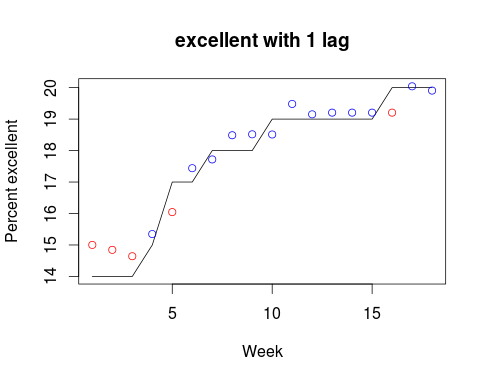
\includegraphics[width=0.8\linewidth]{excellentyear15.png}
\caption{A week-by-week forecast over an entire year is not necessarily as helpful as a multiple-week forecast over a shorter time.}
\end{figure}

A full third lag was detrimental to the model, but it is possible that some combination of field conditions in the third lag would be a predictor.  We would like to add more combinations of lags, and perhaps try more ensemble methods in combination with this model, which is something that we were unable to do in this paper, but may boost its predictive ability substantially.  Lastly, predicting further into the future would be a worthy challenge; by making intermediate predictions, any of these models could project further.  Lastly, charting such a prediction over an entire test year may provide more insight into the capabilities of these models.


\section*{Conclusion}
We compared a large number of models, attempting to predict both future corn field conditions and yearly corn yield. There was a substantial amount of variation in different model's ability to forecast time series. This gives a valuable starting point for future work. It was informative to initially try a large variety of models in order to get a better understanding of each of their capabilities on a given data set. Where we were able, we tried several different methods and strategies on each model in order to improve predictive ability. We were able to learn a lot not only about potential relationships between the variables presented in this paper, but also how different models responded very differently to both the same task, and how the same model can perform very well at one type of time series prediction and poorly in another. 
\end{document}
